
%(BEGIN_QUESTION)
% Copyright 2013, Tony R. Kuphaldt, released under the Creative Commons Attribution License (v 1.0)
% This means you may do almost anything with this work of mine, so long as you give me proper credit

Determine the on/off state of the transistors within this TTL ``NAND'' logic gate, given the input switch states shown in the diagram:

$$\includegraphics[width=15.5cm]{i02091x01.eps}$$

Place one check-mark in each row of the table, identifying the state of each transistor listed:

% No blank lines allowed between lines of an \halign structure!
% I use comments (%) instead, so that TeX doesn't choke.

$$\vbox{\offinterlineskip
\halign{\strut
\vrule \quad\hfil # \ \hfil & 
\vrule \quad\hfil # \ \hfil & 
\vrule \quad\hfil # \ \hfil \vrule \cr
\noalign{\hrule}
%
% First row
{\bf Transistor} & {\bf On} (conducting) & {\bf Off} (non-conducting) \cr
%
\noalign{\hrule}
%
% Another row
$Q_2$ &  &  \cr
%
\noalign{\hrule}
%
% Another row
$Q_3$ &  &  \cr
%
\noalign{\hrule}
%
% Another row
$Q_4$ &  &  \cr
%
\noalign{\hrule}
%
% Another row
$Q_5$ &  &  \cr
%
\noalign{\hrule}
} % End of \halign 
}$$ % End of \vbox

\underbar{file i02091}
%(END_QUESTION)





%(BEGIN_ANSWER)

% No blank lines allowed between lines of an \halign structure!
% I use comments (%) instead, so that TeX doesn't choke.

$$\vbox{\offinterlineskip
\halign{\strut
\vrule \quad\hfil # \ \hfil & 
\vrule \quad\hfil # \ \hfil & 
\vrule \quad\hfil # \ \hfil \vrule \cr
\noalign{\hrule}
%
% First row
{\bf Transistor} & {\bf On} (conducting) & {\bf Off} (non-conducting) \cr
%
\noalign{\hrule}
%
% Another row
$Q_2$ &  & $\surd$ \cr
%
\noalign{\hrule}
%
% Another row
$Q_3$ & $\surd$ &  \cr
%
\noalign{\hrule}
%
% Another row
$Q_4$ & $\surd$ &  \cr
%
\noalign{\hrule}
%
% Another row
$Q_5$ &  & $\surd$ \cr
%
\noalign{\hrule}
} % End of \halign 
}$$ % End of \vbox

%(END_ANSWER)





%(BEGIN_NOTES)

{\bf This question is intended for exams only and not worksheets!}.

%(END_NOTES)

